\section{Random Walk}

\subsection{1D random walk}

\begin{center}
    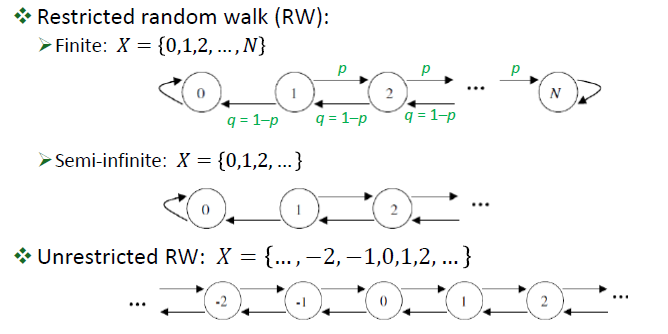
\includegraphics[width=300pt]{images/random walk types.png}
\end{center}

\begin{center}
    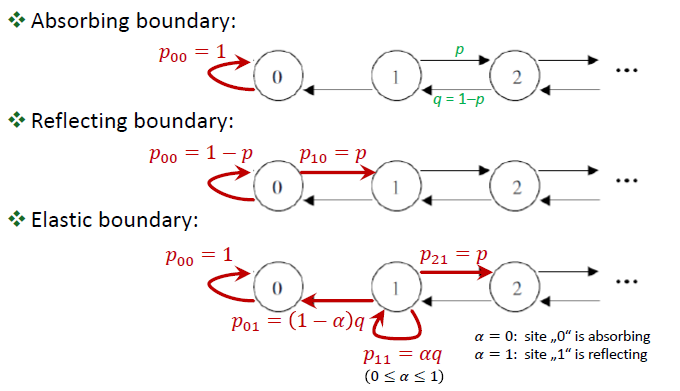
\includegraphics[width=300pt]{images/random walk boundary conditions.png}
\end{center}

\begin{center}
    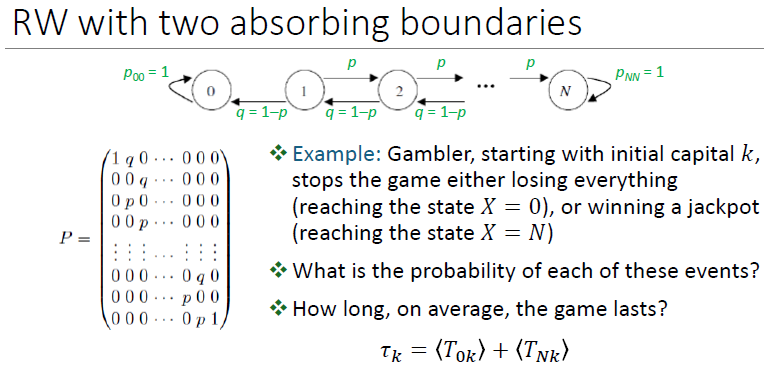
\includegraphics[width=300pt]{images/example rw two absorbing boundaries.png}
\end{center}

Define the probability to lose after $n$ steps by starting from state $k$: $a_{nk} = {\rm Pr} \{ X_n = 0 | X_0 = k \}$ and the probability to win after $n$ steps: $b_{nk} = {\rm Pr} \{ X_n = N | X_0 = k \}$

Then the boundary conditions are

\begin{equation*}
    a_{n0} = 1, \quad a_{nN} = 0, \quad b_{n0} = 0, \quad b_{nN} = 1 
\end{equation*}

Combined probability to end the game after $n$ steps is $a_{nk} + b_{nk}$, hence

\begin{equation*}
    \sum_{n=0}^{\infty} (a_{nk} + b_{nk}) = 1
\end{equation*}

The total probability to lose is $a_k = \sum_{n=0}^{\infty} a_{nk}$

The total probability to win is $b_k = \sum_{n=0}^{\infty} b_{nk}$

The mean duration of the game is $\tau_k = \sum_{n=0}^{\infty} n \cdot (a_{nk} + b_{nk})$

Having defined the essential variables, we can determine the rationship between $a_k$, $a_{k-1}$ and $a_{k+1}$ then
\begin{equation*}
    a_{k} = p a_{k+1} + q a_{k-1}
\end{equation*}
Which means that if you start at state $k$ then you can only move right or left, if you move to state $k+1$ (with probability $p$) then your total probability of losing will be $p a_{k+1}$. Similarly, with moving left.
We obtain a linear second-order homogeneous difference equation in terms of $a_k$:
\begin{equation*}
    pa_{k+1} - a_k + q a_{k-1} = 0
\end{equation*}

To solve this solution we always use the ansatz $a_k = \lambda^{k} \neq 0$

\begin{equation*}
    p \lambda^{k+1} - \lambda^{k} + q \lambda^{k-1} = 0 \quad \Rightarrow \quad \lambda_{1} = 1 \text{ and } \lambda_{2} = \frac{q}{p}
\end{equation*}

\begin{center}
    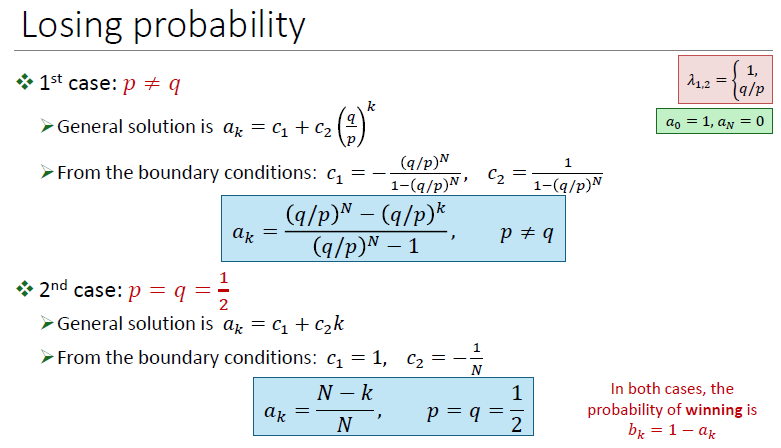
\includegraphics[width=300pt]{images/random walk losing probability.png}
\end{center}

\subsection{Mean duration of game}

Similarly we can write an equation which ties mean duration times, but now notice that we must account for the extra step we did (since we count steps)

\begin{equation*}
    \tau_k = p (1+ \tau_{k+1}) + q(1+ \tau_{k-1}) \quad \Rightarrow \quad p \tau_{k+1} - \tau_{k} + q \tau_{k-1} = -1
\end{equation*}

This is a \textbf{nonhomogeneous} second order difference equation with boundary conditions $\tau_0 = \tau_N = 0$.

We split the solution into two parts: general homogeneous solution $\bar{\tau}_k$ and a particular solution of the nonhomogeneous equation $\tilde{\tau}_k$.

\begin{equation*}
\tau_k = \bar{\tau}_k + \tilde{\tau}_k    
\end{equation*}

We seek a solution of the form
\begin{equation*}
\tau_k = \lambda^k \neq 0.    
\end{equation*}


The characteristic equation gives
\begin{equation*}
\lambda_{1,2} = \{1,\; q/p\}.    
\end{equation*}


\textbf{1st case:} $p \neq q$ \qquad $\tilde{\tau}_k = c\,k$

\begin{equation*}
\tau_k = c_1 + c_2\left(\frac{q}{p}\right)^k + \frac{k}{q - p}
\end{equation*}

or equivalently,

\begin{equation*}
\tau_k = \frac{1}{q - p} 
\left[ k - N \frac{1 - \left(\frac{q}{p}\right)^k}{1 - \left(\frac{q}{p}\right)^N} \right]
\end{equation*}


\textbf{2nd case:} $p = q = \tfrac{1}{2}$ \qquad $\tilde{\tau}_k = c\,k^2$

\begin{equation*}
\tau_k = c_1 + c_2 k - k^2 = k(N - k).    
\end{equation*}


\subsection{Probability distribution}

We have determined the \textbf{total} losing and winning probabilities, but we have not determined the probabilities for seperate events $a_{nk}$ and $b_{nk}$. We can determine them with generating functions

\begin{equation*}
    A_k (s) = \sum_{n=0}^{\infty} a_{nk} s^{n} \qquad \text{and} \qquad B_k(s) = \sum_{n=0}^{\infty} b_{nk} s^{n}
\end{equation*}

\begin{equation}
a_{nk}= \frac{1}{n!}\left.\frac{d^n A_k(s)}{ds^n} \right|_{s=0},
\qquad
b_{nk}= \frac{1}{n!} \left. \frac{d^n B_k(s)}{ds^n}\right|_{s=0}
\end{equation}

\begin{equation}
\tau_k = A_k'(1) + B_k'(1)
\end{equation}

To derive the relations for these values we again can take the known relation for $a$
\begin{equation*}
    a_{n+1,k} = pa_{n, k+1} + q a_{n, k-1}
\end{equation*}

Multiply by $s^{n+1}$ and sum up to obtain

\begin{equation*}
    A_k(s) = ps A_{k+1} + qs A_{k-1}
\end{equation*}

Again we use the same ansatz $A_{k} = [\lambda(s)]^k$. General solution is $A_k(s) = c_1 lambda_1^k + c_2 \lambda_2^{k}$, with boundary conditions $A_0(s) = 1$ and $A_N(s) = 0$. Plugging everything in we obtain

\begin{equation*}
    A_k(s) = \frac{\lambda_1^N \lambda_2^k - \lambda_2^N \lambda_1^k}{\lambda_1^N - \lambda_2^N}
\end{equation*}

Semi-infinite random walk (where there is not cap on winning) can be obtained with the limit $N \rightarrow \infty$. For unrestricted random walk starting from any site, one will \textbf{always} return to this site:
\begin{equation*}
    \sum_{n=1}^{\infty} f_{00}^{(n)} = \frac{1}{2} (a_1 + a_{-1}) = 1
\end{equation*}

However on average the time will be infinite
\begin{equation*}
    \langle T_{00} \rangle = 1 + \tau_1 = 1 + \frac{1}{q-p} = \infty
\end{equation*}